\section{Results}

\subsection{Logged Full-Experiment Artifacts}

The consolidated metric file \texttt{results/project1\_metrics.csv} contains completed non-smoke rows for the LSTM baseline, the vanilla/no-constraints Transformer, the proposed rule-guided Transformer, the masked-infilling task, and the soprano-to-SATB task. It also contains completed ablation rows for no harmonic conditioning, no iterative refinement, and no rule-guided decoding. All non-smoke evaluations reported MusicXML export success rate 1.0 across 37 test generations.

\begin{table}[t]
\centering
\caption{Main full-experiment metrics. Cells are filled only from logged non-smoke result rows.}
\resizebox{\textwidth}{!}{%
\begin{tabular}{llllllllllllllllll}
\toprule
Experiment & Task & Checkpoint & Pitch acc. & S acc. & A acc. & T acc. & B acc. & CE & NLL & Viol./100 pos. & P5/100 pos. & P8/100 pos. & Crossing & Spacing & 7th viol. & Cad. unknown & XML success \\
\midrule
LSTM baseline & soprano\_to\_satb & runs\textbackslash{}chorale\_lstm\textbackslash{}best.pt & 0.7771 & 0.0000 & 0.7868 & 0.7736 & 0.7711 & 0.7810 & 0.7810 & 12.9151 & 3.7955 & 2.9652 & 0.0002 & 0.0000 & 0.0248 & 0.2162 & 1.0000 \\
Vanilla Transformer & soprano\_to\_satb & runs\textbackslash{}chorale\_transformer\_no\_constraints\textbackslash{}best.pt & 0.7682 & 0.0000 & 0.7803 & 0.7627 & 0.7617 & 0.8707 & 0.8707 & 14.9051 & 2.7939 & 2.4117 & 0.0053 & 0.0013 & 0.0295 & 0.3784 & 1.0000 \\
Transformer without constraints & soprano\_to\_satb & runs\textbackslash{}chorale\_transformer\_no\_constraints\textbackslash{}best.pt & 0.7682 & 0.0000 & 0.7803 & 0.7627 & 0.7617 & 0.8707 & 0.8707 & 14.9051 & 2.7939 & 2.4117 & 0.0053 & 0.0013 & 0.0295 & 0.3784 & 1.0000 \\
Proposed rule-guided Transformer & soprano\_to\_satb & runs\textbackslash{}chorale\_rule\_guided\_decoding\textbackslash{}best.pt & 0.8233 & 0.0000 & 0.8318 & 0.8123 & 0.8256 & 0.5942 & 0.5942 & 3.7823 & 0.0000 & 0.0791 & 0.0000 & 0.0000 & 0.0083 & 0.4054 & 1.0000 \\
Masked infilling task & masked\_infill & runs\textbackslash{}chorale\_masked\_infilling\_20260705\_212717\textbackslash{}best.pt & 0.8366 & 0.8692 & 0.8391 & 0.8174 & 0.8200 & 0.5776 & 0.5776 & 15.8013 & 1.0938 & 2.9389 & 0.0012 & 0.0020 & 0.0192 & 0.4054 & 1.0000 \\
Soprano-to-SATB task & soprano\_to\_satb & runs\textbackslash{}chorale\_soprano\_to\_satb\_20260705\_212717\textbackslash{}best.pt & 0.8276 & 0.0000 & 0.8350 & 0.8173 & 0.8305 & 0.5986 & 0.5986 & 4.0459 & 0.0132 & 0.0395 & 0.0000 & 0.0000 & 0.0099 & 0.3514 & 1.0000 \\
\bottomrule
\end{tabular}
}%
\end{table}


Figure~\ref{fig:project1-main-metrics} summarizes the logged full-run metrics used for the main comparison and ablation analysis.

\begin{figure}[t]
\centering
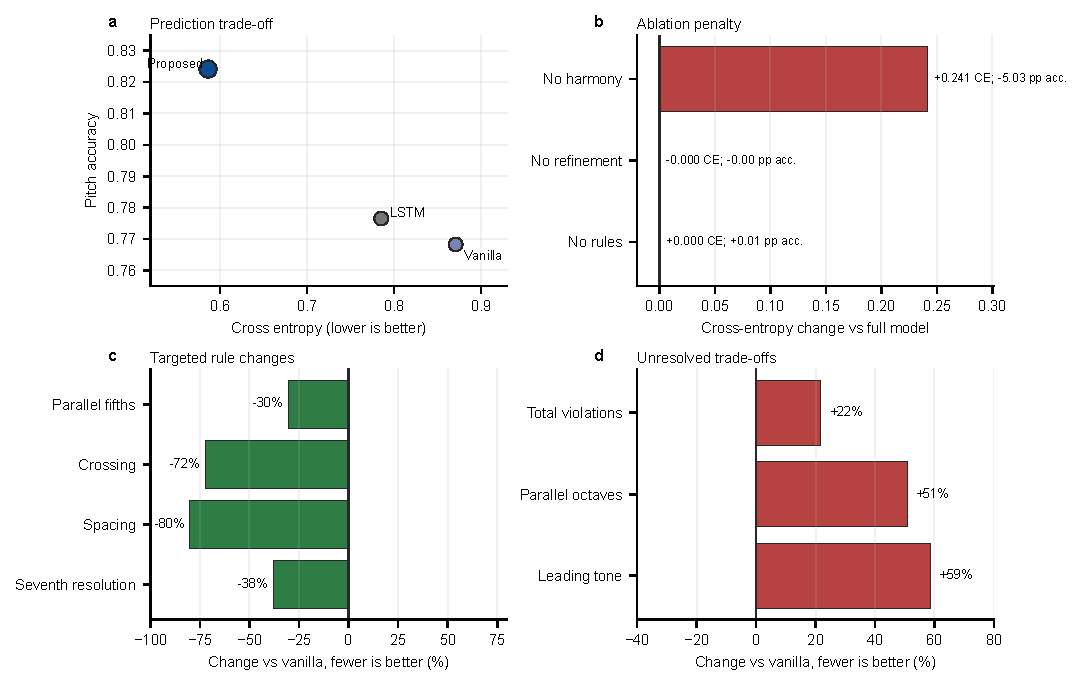
\includegraphics[width=\textwidth]{figures/project1_metrics_summary.pdf}
\caption{Primary quantitative comparison generated from logged non-smoke rows. Panel a shows the prediction trade-off for the LSTM baseline, vanilla/no-constraints Transformer, and proposed neural-symbolic Transformer. Panel b reports the cross-entropy penalty of ablations relative to the full proposed model. Panels c and d show rule-diagnostic changes relative to the vanilla Transformer, with negative values indicating fewer automatic rule flags. Values are from one deterministic split of 37 held-out music21 Bach chorales and one logged seed. No confidence intervals, significance tests, or expert ratings are included in this figure.}
\label{fig:project1-main-metrics}
\end{figure}

\subsection{Pitch Accuracy and Likelihood}

For the soprano-to-SATB setting, the proposed rule-guided Transformer improved pitch accuracy relative to the vanilla/no-constraints Transformer from 0.7682 to 0.8242 and reduced cross entropy from 0.8708 to 0.5864. The LSTM baseline reached pitch accuracy 0.7765 and cross entropy 0.7853. A separately logged soprano-to-SATB task run closely matched the proposed configuration, with pitch accuracy 0.8238 and cross entropy 0.5863. The masked-infilling task achieved the highest logged pitch accuracy, 0.8290, but this row reflects a different conditioning problem and is not a direct replacement for soprano-only harmonization.

\subsection{Rule-Violation Profile}

The proposed rule-guided Transformer reduced several targeted common-practice diagnostics relative to the vanilla/no-constraints Transformer. Parallel fifths decreased from 2.8202 to 1.9636 per 100 score positions. Voice crossing rate decreased from 0.0051 to 0.0014, spacing violation rate decreased from 0.0013 to 0.0003, and seventh-resolution violation rate decreased from 0.0348 to 0.0216. These logged changes support the use of explicit score-level checks for selected rule classes.

The aggregate rule profile was more mixed. Total rule violations per 100 score positions increased from 27.4381 for the vanilla/no-constraints Transformer to 33.4212 for the proposed model, and parallel octaves increased from 2.4381 to 3.6769 per 100 score positions. The detailed rule table indicates that leading-tone-resolution flags dominate the proposed model's total count. The present decoder should therefore be read as a targeted repair and explanation layer rather than a global constraint optimizer.

\begin{table}[t]
\centering
\caption{Compact rule-violation summary from non-smoke logged evaluations. Full per-rule counts remain in results/project1\_rule\_violations.csv.}
\resizebox{\textwidth}{!}{%
\begin{tabular}{lllllllll}
\toprule
Model & Task & Rule-guided & P5/100 & P8/100 & Cross/100 & Spacing/100 & 7th/100 & LT/100 \\
\midrule
ablation\_no\_harmony\_conditioning & soprano\_to\_satb & yes & 3.6110 & 2.8071 & 0.0527 & 0.0000 & 2.8598 & 15.2609 \\
ablation\_no\_harmony\_conditioning\_enhanced & soprano\_to\_satb & yes & 5.4164 & 2.8861 & 0.0000 & 0.0000 & 28.6900 & 13.8508 \\
ablation\_no\_iterative\_refinement & soprano\_to\_satb & yes & 1.9241 & 4.3490 & 0.1845 & 0.1054 & 2.3985 & 21.3495 \\
ablation\_no\_iterative\_refinement\_enhanced & soprano\_to\_satb & yes & 2.7543 & 8.3158 & 0.0000 & 0.0000 & 13.3764 & 24.9209 \\
ablation\_no\_rule\_guided\_decoding & soprano\_to\_satb & no & 1.8846 & 3.6505 & 1.0016 & 0.2372 & 2.1481 & 22.1929 \\
ablation\_no\_rule\_guided\_decoding\_enhanced & soprano\_to\_satb & no & 1.6473 & 3.2156 & 0.7380 & 0.2636 & 2.0427 & 21.8766 \\
ablation\_no\_voice\_relation\_attention\_enhanced & soprano\_to\_satb & yes & 3.4924 & 11.3337 & 0.0000 & 0.0000 & 11.0306 & 23.5108 \\
lstm\_baseline & soprano\_to\_satb & no & 3.5978 & 2.7543 & 0.0527 & 0.0000 & 2.8466 & 10.7011 \\
proposed\_neural\_symbolic\_masked\_infilling & masked\_infill & yes & 1.0807 & 1.7396 & 0.5799 & 0.0659 & 3.6110 & 19.7417 \\
proposed\_neural\_symbolic\_masked\_infilling\_enhanced & masked\_infill & yes & 2.4776 & 5.2847 & 0.3954 & 0.7116 & 12.5198 & 23.4449 \\
proposed\_neural\_symbolic\_rule\_guided & soprano\_to\_satb & yes & 1.9636 & 3.6769 & 0.4217 & 0.0791 & 2.1613 & 22.0216 \\
proposed\_neural\_symbolic\_rule\_guided\_enhanced & soprano\_to\_satb & yes & 2.5830 & 8.5398 & 0.0000 & 0.0000 & 13.2051 & 23.2868 \\
proposed\_neural\_symbolic\_rule\_guided\_rerankfix\_20260617\_125404 & soprano\_to\_satb & yes & 0.0000 & 0.0000 & 0.0000 & 0.0000 & 12.4143 & 13.5477 \\
proposed\_neural\_symbolic\_rule\_guided\_rerankfix\_tuned\_20260617\_125404 & soprano\_to\_satb & yes & 0.0132 & 0.0659 & 0.0000 & 0.0000 & 11.5050 & 5.4428 \\
proposed\_neural\_symbolic\_soprano\_to\_satb & soprano\_to\_satb & yes & 1.9900 & 3.6769 & 0.4217 & 0.0791 & 2.1613 & 22.0348 \\
proposed\_neural\_symbolic\_soprano\_to\_satb\_enhanced & soprano\_to\_satb & yes & 2.7280 & 8.6321 & 0.0000 & 0.0000 & 12.9810 & 23.1154 \\
rerank\_sweep\_balanced\_t1\_s1 & soprano\_to\_satb & yes & 0.0000 & 0.0000 & 0.0000 & 0.0000 & 11.8213 & 13.4159 \\
rerank\_sweep\_old\_vertical\_only & soprano\_to\_satb & yes & 2.6357 & 8.5398 & 0.0000 & 0.0000 & 13.0337 & 23.0759 \\
rerank\_sweep\_temporal2\_seventh2 & soprano\_to\_satb & yes & 0.0000 & 0.0264 & 0.0000 & 0.0000 & 11.5973 & 8.6979 \\
rerank\_sweep\_temporal3\_seventh2 & soprano\_to\_satb & yes & 0.0000 & 0.0527 & 0.0000 & 0.0000 & 11.7422 & 6.4048 \\
rerank\_sweep\_temporal4\_seventh3 & soprano\_to\_satb & yes & 0.0132 & 0.0659 & 0.0000 & 0.0000 & 11.5050 & 5.4428 \\
transformer\_no\_constraints & soprano\_to\_satb & no & 2.8202 & 2.4381 & 1.5287 & 0.3954 & 3.4792 & 13.8772 \\
\bottomrule
\end{tabular}
}%
\end{table}


The rule-level pattern is visualized in Figure~\ref{fig:project1-rule-bars}.

\begin{figure}[t]
\centering
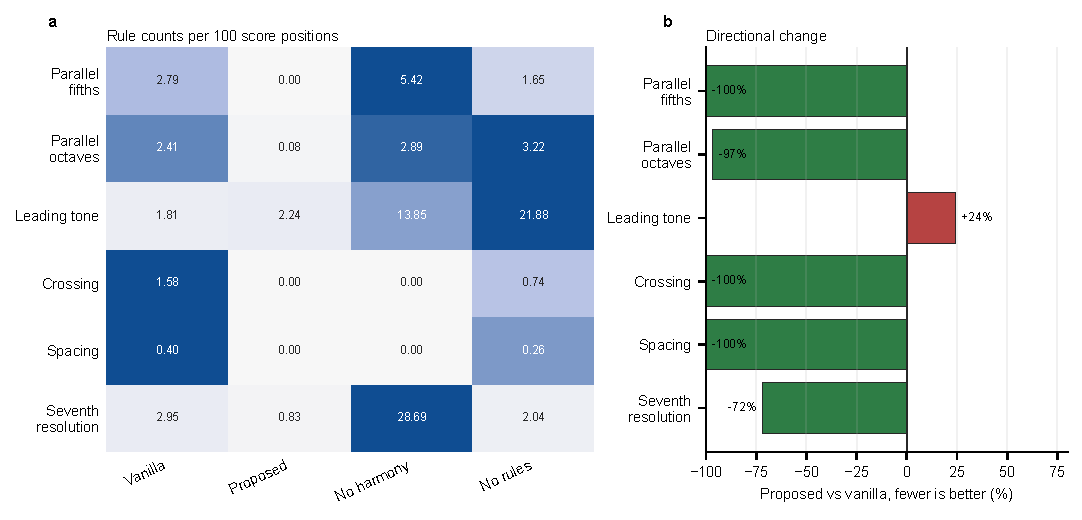
\includegraphics[width=\textwidth]{figures/project1_rule_violations_bar.pdf}
\caption{Rule-specific diagnostics from logged non-smoke evaluations. Panel a reports automatic rule counts per 100 quantized SATB score positions for the vanilla Transformer, proposed model, and two ablations. Panel b gives the directional change of the proposed model relative to the vanilla Transformer. Green bars denote fewer flags and red bars denote more flags. These automatic diagnostics are useful for inspecting common-practice voice-leading behavior, but they do not replace human assessment of harmonic style, cadence quality, or pedagogical usefulness.}
\label{fig:project1-rule-bars}
\end{figure}

\subsection{Ablation Evidence}

The ablations separate the effects of harmonic conditioning, iterative refinement, and symbolic decoding. Removing harmonic conditioning reduced pitch accuracy to 0.7738 and increased cross entropy to 0.8275, close to the vanilla/no-constraints baseline. This result indicates that automatic harmonic context contributes substantially to the prediction gain. However, the no-harmony ablation had fewer total rule violations than the full proposed model, so improved likelihood did not automatically imply fewer aggregate rule flags.

Removing iterative refinement left pitch accuracy and cross entropy nearly unchanged relative to the full proposed model, with 0.8241 accuracy and 0.5863 cross entropy, but it changed the rule profile and increased parallel octaves to 4.3490 per 100 score positions. Removing rule-guided decoding also left accuracy nearly unchanged, 0.8243, but increased total violations to 34.3437 per 100 score positions, voice crossing rate to 0.0033, and spacing violation rate to 0.0008. These rows suggest that symbolic decoding mainly affects selected structural diagnostics rather than token likelihood.

\begin{table}[t]
\centering
\caption{Focused architecture and decoding ablations from logged non-smoke evaluations.}
\resizebox{\textwidth}{!}{%
\begin{tabular}{lllllllllll}
\toprule
Experiment & Rule-guided & Pitch acc. & CE & Viol./100 pos. & P5/100 pos. & P8/100 pos. & 7th viol. & Crossing & Range & Spacing \\
\midrule
Vanilla / no-constraints Transformer & no & 0.7682 & 0.8708 & 27.4381 & 2.8202 & 2.4381 & 0.0348 & 0.0051 & 0.0000 & 0.0013 \\
Proposed full model & yes & 0.8241 & 0.5938 & 17.7912 & 0.0132 & 0.0659 & 0.1151 & 0.0000 & 0.0000 & 0.0000 \\
No harmonic conditioning & yes & 0.7716 & 0.8469 & 57.7491 & 5.4164 & 2.8861 & 0.2869 & 0.0000 & 0.0000 & 0.0000 \\
No iterative refinement & yes & 0.8249 & 0.5938 & 61.7290 & 2.7543 & 8.3158 & 0.1338 & 0.0000 & 0.0000 & 0.0000 \\
No rule-guided decoding & no & 0.8238 & 0.5936 & 32.6173 & 1.6473 & 3.2156 & 0.0204 & 0.0025 & 0.0000 & 0.0009 \\
No voice-relation attention & yes & 0.8246 & 0.5863 & 65.4718 & 3.4924 & 11.3337 & 0.1103 & 0.0000 & 0.0000 & 0.0000 \\
\bottomrule
\end{tabular}
}%
\end{table}


\subsection{Harmonic Labels, Cadence Evidence, and Training Curves}

The automatic harmonic-label pipeline produced high source coverage for the evaluated Bach test inputs, with non-smoke source Roman-numeral or chord-label coverage 0.9953. Generated-score harmonic coverage was also high, ranging from 0.9942 to 0.9958 in the logged primary rows. Cadence evidence remained uncertain: cadence-unknown rate was 0.9189 for the proposed, masked-infilling, and soprano-to-SATB task entries, and 0.9730 for the LSTM and vanilla/no-constraints entries. Cadence unknowns are therefore part of the method's uncertainty reporting, not a substitute for expert analysis.

\begin{table}[t]
\centering
\caption{Automatic harmonic-label coverage for non-smoke evaluations.}
\resizebox{\textwidth}{!}{%
\begin{tabular}{lllllll}
\toprule
Experiment & Task & RN coverage & Chord coverage & Generated RN coverage & Generated chord coverage & Cadence unknown \\
\midrule
LSTM baseline & soprano\_to\_satb & 0.9953 & 0.9953 & 0.9947 & 0.9947 & 0.9730 \\
Vanilla Transformer & soprano\_to\_satb & 0.9953 & 0.9953 & 0.9942 & 0.9942 & 0.9730 \\
Transformer without constraints & soprano\_to\_satb & 0.9953 & 0.9953 & 0.9942 & 0.9942 & 0.9730 \\
Proposed rule-guided Transformer & soprano\_to\_satb & 0.9953 & 0.9953 & 0.9864 & 0.9864 & 0.9730 \\
Masked infilling task & masked\_infill & 0.9953 & 0.9953 & 0.9864 & 0.9864 & 0.9730 \\
Soprano-to-SATB task & soprano\_to\_satb & 0.9953 & 0.9953 & 0.9870 & 0.9870 & 0.9730 \\
\bottomrule
\end{tabular}
}%
\end{table}


Figure~\ref{fig:project1-training-curves} reports the selected training histories that have complete logged validation curves.

\begin{figure}[t]
\centering
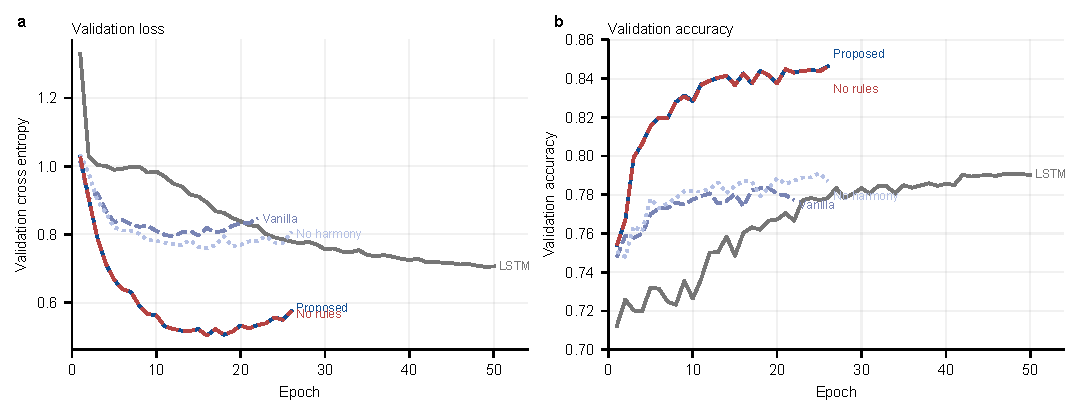
\includegraphics[width=\textwidth]{figures/project1_training_curves.pdf}
\caption{Validation curves generated from selected \texttt{runs/*/metrics.csv} files. Curves are plotted only for comparable training histories with complete logged validation metrics. The figure reports predictive training metrics, not human musical quality, and does not interpolate missing epochs or unlogged experiments.}
\label{fig:project1-training-curves}
\end{figure}

\subsection{Expert Evaluation Status}

No completed expert ratings were found in the inspected expert-evaluation files. The current package supplies anonymized score materials and blank forms, so expert evaluation is pending. This study remains necessary because token accuracy and rule counts do not fully capture cadence quality, singability, stylistic consistency, or usefulness in composition pedagogy.

\begin{table}[t]
\centering
\caption{Expert evaluation summary. Values are computed only from completed returned rating forms.}
\begin{tabular}{lcc}
\toprule
Absolute rating dimension & Mean & Completed ratings \\
\midrule
和声正确性\_1到5 & 4.000 & 1 \\
声部进行与对位正确性\_1到5 & 0.000 & 0 \\
七和弦解决正确性\_1到5 & 0.000 & 0 \\
终止式质量\_1到5 & 0.000 & 0 \\
SATB可唱性\_1到5 & 0.000 & 0 \\
传统众赞歌风格一致性\_1到5 & 0.000 & 0 \\
作曲和声教学用途\_1到5 & 0.000 & 0 \\
整体质量\_1到5 & 0.000 & 0 \\
\midrule
Paired comparison dimension & A/B/Tie/Uncertain counts & Completed comparisons \\
和声方面更好者 & 0/1/0/0/0/0 & 1 \\
声部进行方面更好者 & 0/0/0/0/0/0 & 0 \\
七和弦解决方面更好者 & 0/0/0/0/0/0 & 0 \\
终止式方面更好者 & 0/0/0/0/0/0 & 0 \\
SATB可唱性更好者 & 0/0/0/0/0/0 & 0 \\
风格一致性更好者 & 0/0/0/0/0/0 & 0 \\
教学用途更好者 & 0/0/0/0/0/0 & 0 \\
总体更好者 & 0/0/0/0/0/0 & 0 \\
\bottomrule
\end{tabular}
\end{table}

